\def\year{2020}
%File: main.tex
\documentclass[letterpaper]{article} % DO NOT CHANGE THIS
\usepackage{aaai20}  % DO NOT CHANGE THIS
\usepackage{times}  % DO NOT CHANGE THIS
\usepackage{helvet} % DO NOT CHANGE THIS
\usepackage{courier}  % DO NOT CHANGE THIS
\usepackage[hyphens]{url}  % DO NOT CHANGE THIS
\usepackage{graphicx} % DO NOT CHANGE THIS
\usepackage{algorithm}
\usepackage{algpseudocode}
\usepackage{float}
\usepackage{subfig}
\urlstyle{rm} % DO NOT CHANGE THIS
\def\UrlFont{\rm}  % DO NOT CHANGE THIS
\usepackage{graphicx}  % DO NOT CHANGE THIS
\usepackage{xcolor}
\usepackage{amssymb}
\usepackage{mathtools}
%\usepackage{pcatcode}


\usepackage{amsthm}

\theoremstyle{definition}
\newtheorem{definition}{Definition}
%\newtheorem{definition}{Definition}[section]

\frenchspacing  % DO NOT CHANGE THIS
\setlength{\pdfpagewidth}{8.5in}  % DO NOT CHANGE THIS
\setlength{\pdfpageheight}{11in}  % DO NOT CHANGE THIS

\newtheorem{example}{Example}

\newcommand{\commentout}[1]{}
\newcommand{\eliran}[1]{\textbf{[\color{red}ELIRAN:#1]}}
\newcommand{\ronen}[1]{\textbf{[\color{blue}RONEN:#1]}}
\newcommand{\guy}[1]{\textbf{[\color{orange}GUY:#1]}}
%\newcommand{\begin{example}}[1]{\textbf{[\color{purple}RunningExample:#1]}}

\newcommand{\cbp}[0]{Collaborative Box-Pushing}
\newcommand{\mitg}[0]{Meet In The Grid}
\newcommand{\crs}[0]{Cooperative Rock-Sampling}
\newcommand{\macor}[0]{Multi-Agent Corridor}

\newcommand{\cact}[1]{{\em CActions$_#1$}}
\newcommand{\mcact}[1]{{\mathit{CActions}_#1}}
\newcommand{\pcact}[1]{{\mathit{PCA}_#1}}
\newcommand{\eff}{\mathit{eff}}

\newcommand{\Tau}{\mathrm{T}}

%\nocopyright
%PDF Info Is REQUIRED.
% For /Author, add all authors within the parentheses, separated by commas. No accents or commands.
% For /Title, add Title in Mixed Case. No accents or commands. Retain the parentheses.
 \pdfinfo{
/Title (A Factored Approach To Solving Dec-POMDPs)
/Author (Eliran Abdoo, Ronen I. Brafman, Guy Shani)
} %Leave this	
% /Title ()
% Put your actual complete title (no codes, scripts, shortcuts, or LaTeX commands) within the parentheses in mixed case
% Leave the space between \Title and the beginning parenthesis alone
% /Author ()
% Put your actual complete list of authors (no codes, scripts, shortcuts, or LaTeX commands) within the parentheses in mixed case. 
% Each author should be only by a comma. If the name contains accents, remove them. If there are any LaTeX commands, 
% remove them. 

% DISALLOWED PACKAGES
% \usepackage{authblk} -- This package is specifically forbidden
% \usepackage{balance} -- This package is specifically forbidden
% \usepackage{caption} -- This package is specifically forbidden
% \usepackage{color (if used in text)
% \usepackage{CJK} -- This package is specifically forbidden
% \usepackage{float} -- This package is specifically forbidden
% \usepackage{flushend} -- This package is specifically forbidden
% \usepackage{fontenc} -- This package is specifically forbidden
% \usepackage{fullpage} -- This package is specifically forbidden
% \usepackage{geometry} -- This package is specifically forbidden
% \usepackage{grffile} -- This package is specifically forbidden
% \usepackage{hyperref} -- This package is specifically forbidden
% \usepackage{navigator} -- This package is specifically forbidden
% (or any other package that embeds links such as navigator or hyperref)
% \indentfirst} -- This package is specifically forbidden
% \layout} -- This package is specifically forbidden
% \multicol} -- This package is specifically forbidden
% \nameref} -- This package is specifically forbidden
% \natbib} -- This package is specifically forbidden -- use the following workaround:
% \usepackage{savetrees} -- This package is specifically forbidden
% \usepackage{setspace} -- This package is specifically forbidden
% \usepackage{stfloats} -- This package is specifically forbidden
% \usepackage{tabu} -- This package is specifically forbidden
% \usepackage{titlesec} -- This package is specifically forbidden
% \usepackage{tocbibind} -- This package is specifically forbidden
% \usepackage{ulem} -- This package is specifically forbidden
% \usepackage{wrapfig} -- This package is specifically forbidden
% DISALLOWED COMMANDS
% \nocopyright -- Your paper will not be published if you use this command
% \addtolength -- This command may not be used
% \balance -- This command may not be used
% \baselinestretch -- Your paper will not be published if you use this command
% \clearpage -- No page breaks of any kind may be used for the final version of your paper
% \columnsep -- This command may not be used
% \newpage -- No page breaks of any kind may be used for the final version of your paper
% \pagebreak -- No page breaks of any kind may be used for the final version of your paperr
% \pagestyle -- This command may not be used
% \tiny -- This is not an acceptable font size.
% \vspace{- -- No negative value may be used in proximity of a caption, figure, table, section, subsection, subsubsection, or reference
% \vskip{- -- No negative value may be used to alter spacing above or below a caption, figure, table, section, subsection, subsubsection, or reference

\setcounter{secnumdepth}{2} %May be changed to 1 or 2 if section numbers are desired.

% The file aaai20.sty is the style file for AAAI Press 
% proceedings, working notes, and technical reports.
%
\setlength\titlebox{2.5in} % If your paper contains an overfull \vbox too high warning at the beginning of the document, use this
% command to correct it. You may not alter the value below 2.5 in
\title{A Factored Approach To Solving Dec-POMDPs }
%Your title must be in mixed case, not sentence case. 
% That means all verbs (including short verbs like be, is, using,and go), 
% nouns, adverbs, adjectives should be capitalized, including both words in hyphenated terms, while
% articles, conjunctions, and prepositions are lower case unless they
% directly follow a colon or long dash
\author{Eliran Abdoo, Ronen I Brafman, Guy Shani\\
Ben-Gurion University, Israel\\
eliranb,brafman,shanigu@bgu.ac.il}
\begin{document}

\maketitle

\begin{abstract}
Dec-POMDPs model planning problems under uncertainty and partial observability for a distributed team of cooperating agents planning together but executing their plans in a distributed manner. This problem is
very challenging computationally (NEXP-Time Complete) and consequently, exact methods have difficulty scaling up. In this paper we present a heuristic approach for solving certain instances of Factored Dec-POMDP. Our approach reduces the joint planning problem to multiple single agent POMDP planning problems.
First, we solve a centralized version of the Dec-POMDP, which we call the team problem, where agents have a shared belief state. Then, each agent individually plans to execute its part of the team plan. Finally, the different solutions are aligned to achieve synchronization. Using this approach we are able to solve larger Dec-POMDP problems, limited mainly by the abilities of the underlying POMDP solver.
\end{abstract}




\section{Introduction}

Decentralized Partially Observable Markov Decision Processes (Dec-POMDPs) are a popular model for planning in stochastic environments under uncertainty with partial observability by a distributed team of agents \cite{DECPOMDPART}. In this model, a team of agents attempts to maximize the team's cumulative reward where each agent has only partial information about the state of the system during execution.  The team can plan together centrally prior to acting, but during execution each agent is aware of its own observations only. Communication is possible only through explicit communication actions, if these are available. 

To achieve their common goal agents must coordinate their actions in two ways: First, as in single agent problems, actions must be coordinated sequentially. That is, current actions must help steer the system later towards states in which greater reward will be possible. For example, to be rewarded for shipping a product, it must first be assembled. 
Second, agents may need to coordinate their simultaneous actions because their effects are dependent, e.g., a heavy box can only be pushed if two agents push it simultaneously. 

Our focus is on centralized off-line planning for distributed execution. That is, offline, a solver with access to the complete model must generate a policy for each agent. An agent's policy specifies which action it executes as a function of the agent's history of
actions and observations. Such policies can be represented by a {\em policy graph} where nodes are labeled by actions, and edges are labeled by observations. Online, each agent executes its own policy independently of the other agents.
The challenge is to generate policies that provide sufficient coordination, even though each agent makes different observations at run-time. Thus, agents' beliefs over which states are possible are typically different. 

Dec-POMDPs are notoriously hard to solve -- they are NEXP-Time hard~\cite{DECPOMDPCOMP}, implying that only the smallest toy problems are optimally solvable.
However, many approximate methods for solving Dec-POMDPs have been proposed, with steady progress. Some of these methods generate solutions with bounds on
their optimality \cite{GMAAICE,MBDP,DICEPS}, and some are heuristic in nature~\cite{JESP}. However, current methods typically do not scale to state spaces with more than a few hundreds of states.


In this paper we describe a heuristic approach for solving Dec-POMDPs that scales to much larger state spaces. The key idea is to solve a Dec-POMDP by
solving multiple POMDPs. First, we solve  the {\em team POMDP}, a POMDP in which every observation by one agent is immediately available to the other agents. Hence, all agents have the same belief state.  The solution of the team
POMDP can be represented by a policy graph --- the {\em team policy graph.} . It provides us with a skeleton for the solution of the Dec-POMDP, specifying what each agent needs to provide for the team. Naturally, this policy is not executable by the agents, because agents cannot condition their actions on the observations of other agents in the real world.

Hence, in the next stage, we let each agent solve a POMDP in which it is rewarded for behaving following the specification in the team policy. This leads to the generation of a policy tree for each agent. 
These policy trees are often not well synchronized. In the last step we synchronize the policy trees by delaying the actions of agents to improve the probability of good coordination. 

We implemented our algorithm and tested it on several configurations of a benchmark problem: \cbp\ which is a variation of the Cooperative Box Pushing problem. We show that the algorithm manages to scale well beyond
current Dec-POMDP solvers.
One of the main properties of the domain, is that agents policies are only loosely coupled. That is, the need for actions that affect state components that are relevant to all agent, is sparse. That sparsity allows for each agent to independently construct a plan that consists mostly of its own private actions without requiring it to consider the other agents' behavior. This allows us to achieve good decentralized policies even when achieving the goal requires many steps, compared to planning directly over the Dec-POMDP model.






\section{Background}

We now provide needed background on POMDPs, Dec-POMDPs, their factored representation, and policies. We also introduce the concept of private and public variables and actions in Dec-POMDPs.


\subsection{POMDPs}

A POMDP is a model for single-agent sequential decision making under uncertainty and partial observability.
Formally, it is a tuple $P=\langle S, A, T, R, \Omega, O, \gamma, h, b_0 \rangle$, where:
\begin{itemize}
\item
$S$ is the set of states. The future is independent of the past, given the current state.
\item
$A$ is the set of actions. An action may modify the state and/or
provide information about the current state.
\item
$T: S \times A \rightarrow \prod(S)$ is the state transition function.  $T(s, a, s')$ is the probability of transitioning to $s'$ when applying $a$ in $s$. 
\item
$R:S \times A \times S \rightarrow \mathbb{R}$  is the immediate reward function. $R(s,a, s')$ is the reward obtained after performing $a$ in $s$  and reaching $s'$. 
\item
$\Omega$ is the set of observations. An observation is obtained by the agent following an action, and provides some  information about the world.
\item
$O:S \times A \rightarrow \prod (\Omega)$ is the observation function, specifying the likelihood of sensing a specific observation following an action. $O(s', a, o)$ is the probability of observing $o\in \Omega$ when performing $a$ and \emph{reaching} $s'$. 
\item
$\gamma \in (0,1)$ is the discount factor, quantifying the relative importance of immediate rewards vs.~future rewards.
\item
$h$ is the planning horizon --- the amount of actions that an agent executes before terminating. The horizon may be infinite.
% \eliran{Open issue - included infinity as our algorithm outputs a policy for infinite horizon, where we state this?}
% \ronen{Do we really plan for an infinite horizon? Perhaps you mean unbounded horizon?}\eliran{I'm not sure actually. The policies we output are for infinite horizons (there's an edge for every possible observation of the node's action), but perhaps it is because we plan for enough steps so that the policy graph closes, and then it might be for an unbounded horizon. I'll look into it}
%\eliran{we said it can be considered as "unbounded horizon", should we drop the $\infty$ sign?}

\item
$b_0\in \prod(S)$ is a distribution over $S$ specifying the probability distribution over the initial state.
\end{itemize}

For ease of representation, we assume that agent actions are either sensing actions or non-sensing actions. An agent that applies a non-sensing action receives the observation {\em null-obs}. In addition, we also assume that every action has 
an effect that we consider as the successful outcome, while all other effects are considered failures. We later explain how this assumption can be omitted in the relevant parts.

Often, the state space $S$ is structured, i.e., it consists of assignments to some set of variables $X_1,\ldots X_k$, and the observation space $\Omega$ is
also structured, consisting of a set of observation variables $W_1,\ldots, W_d$. 
Thus, $S=Dom(X_1)\times\cdots\times Dom(X_k)$ and
$\Omega = Dom(W_1)\times\cdots\times Dom(W_d)$. 
In that case, $\tau$, $O$, and $R$ can be represented compactly by, e.g., a dynamic Bayesian network~\cite{BAYESNETWORK}. Formats such as RDDL~\cite{RDDL} and POMDPX~\cite{POMDPX}
exploit factored representations to specify POMDPs compactly.

\begin{example}
Consider a simple Box-Pushing in a 2 tile grid. The left tile is marked by \emph{L} and the right tile by \emph{R}. The agent begins in the left tile. There is a single box, that starts in the right tile. The agent can either move, sense its current tile or push a box from its current tile. Both move and push can be done in any direction --- left and right. The agent's goal is to push the box to the right tile.
The state is composed of 2 variables: the location of the agent and the location of the box. Each variable can take one of two values: \emph{L} or \emph{R}.
The sense action returns an observation telling whether there's a box in the agent's tile, while the move and push actions are non-sensing actions always returning {\em null-obs}.
The push action has a success probability of 0.8.
\end{example}

A solution to a POMDP can be formed as a {\em policy}, assigning to each history of actions and observation ({\em $AO$-history}) the next action to execute. 
Such a policy is often represented using a {\em policy tree} or, more generally, a {\em policy graph} (also called a finite-state controller). 

A policy graph $G=(V,E)$ is a directed simple graph, in which each vertex is associated with an action, and each edge is associated with an observation.
For every edge $v\in V$ and every observation $o\in\Omega$ exactly one edge emanates from $v$ with the label $o$.
The graph has a single root which acts as its entry point. Every $AO$-history $h$ can be associated with some path from the root to some vertex $v$,
and the action labelling $v$ is the action that the policy associates with $h$.

Finally, using a policy graph to direct the agent on the problem produces a {\em trace} -- an execution trajectory. A trace $T$ of length $l$ is a sequence of quintuplets $e_i = (s_i, a_i, s'_i, o_i, r_i)$, namely \emph{steps}, that occurred during a possible policy execution where: $s_i$ is a state in step $i$ and $s_0$ is the initial state;
$a_i$ is the action taken in step $i$;
    $s'_i$ is the result of applying $a_i$ in $s_i$;
    $o_i$ is the observation received after taking $a_i$ and reaching $s'_i$; and is the reward received for taking the $a_i$ in $s_i$ and reaching $s'_i$. Clearly, $\forall i$ such
    that $0\leq i \leq l-1$, we have $s'_i=s_{i+1}$.




\subsection{Dec-POMDP}

A Dec-POMDP models problems where there are $n>1$ acting agents.. 
These agents are part of a team, sharing the same reward, but they act in a distributed manner,
sensing different observations. Thus, their information state is often different. 
Formally, a Dec-POMDP for $n$ agents is a tuple  $P=(S, A=\bigcup_{i=1}^{n}{\{A_i\}}, T, R, \Omega=\bigcup_{i=1}^{n}{\{\Omega_i\}},  O, \gamma, h, {\{I_i\}}_{i=1}^{n})$, where:
\begin{itemize}
\item
$S,\gamma,h,b_0$ are defined as in a POMDP.
\item
$A_i$ is the set of actions available to agent $i$. We assume that $A_i$ contains a special {\em no-op} action, which does not change the state of the world, and does not provide any informative observation. 
$A=A_1 \times A_2 \times .. \times A_n$ is the set of joint actions. On every step each agent $i$ chooses an action $a_i \in A_i$ to execute, and all agents execute their actions jointly. $\langle a_1,...,a_n \rangle$ is known as a joint action. We often treat the
single-agent action $a_i$ as a joint-action, with the understanding that it refers to the joint-action $\langle$no-op,$\ldots,a_i,\ldots,$no-op$\rangle$
\item
$T:S \times A \rightarrow \prod(S)$  is the transition function. Transitions are specified for joint actions, that is, $T(s, \langle a_1,...,a_n \rangle, s')$ is the probability of transitioning from state $s$ to state $s'$ when each agent $i$ executes action $a_i$.
\item
$R:S \times A \times S \rightarrow \mathbb{R}$  is the reward function. Rewards are also specified over joint actions.
\item
$\Omega = \Omega_1 \times \Omega_2 \times .. \times \Omega_n$ is the set of joint observations. Each $\Omega_i$ contains a special {\em null-obs} observation received when applying a non-sensing action.
\item
$O:S \times A \rightarrow \prod_{i=1..n}(\Omega_i)$  is the observation function, specified over joint actions. $O(s',\langle a_1,...,a_n \rangle,\langle o_1,...,o_n \rangle)$ is the probability that when all agents execute $\langle a_1,...,a_n \rangle$ jointly and reach $s'$, each agent $i$ observes $o_i$.
\item
$\gamma$  is the discount factor.
\item
$h$ is the horizon.
\item
$b_0 \in \prod(S)$ is a distribution over $S$ specifying the probability that each agent begin its execution in each state. In principle, different agents may have different initial belief states, but
we make the (common) assumption that the initial belief state is identical. 
\end{itemize}



\begin{example}
We extend the previous example 
to a Dec-POMDP by adding an agent at the right tile and a second box that starts in the left tile. The agents are denoted by \emph{Agent1} and \emph{Agent2} and the boxes by \emph{Box1}, and \emph{Box2}. \emph{Box1} must reach the left tile, and \emph{Box2} must reach the right tile.
\end{example}

As in the case of POMDPs, Dec-POMDPs can also be represented in a factored manner \cite{FDECPOMDP}, although most work to date uses the flat-state representation.
%(e.g., \cite{GMAAICE}, \cite{JESP}).
We add the notion of \emph{observation variables}, which capture the observation value of each agent following an action. Each observation variable is denoted by $\omega_i$ which takes values in $\Omega_i$, and represents the observation of agent $i$.

\begin{example}
In our example, the state is now composed of 4 state variables: the location of each box -- $(X_{B1}, X_{B2})$ -- and the location of each agent -- $(X_{A1}, X_{A2})$. In addition, there are two observation variables -- $(\omega_1, \omega_2)$.
\end{example}

An important element of a factored specification of Dec-POMDPs is a compact formalism for specifying joint-actions. If there are $|A|$ actions in the domain, then, in principle, there are $O(|A|^n)$ possible joint actions. Specifying all joint actions explicitly is unrealistic for large domains. 

In many problems of interest we may expect
that most actions will not interact with each other. A pair of actions $a\in A_i$, $a' \in A_j$ is said to be non interacting, if their effects when applied jointly (in the same joint action) is the union of their effects when applied separately.
Thus, our specification language focuses on specifying
the effects of single-agent actions and specific
combinations of single-agent actions that interact with each other, which we refer to as {\em collaborative} actions~\cite{IMAP}.
For a more detailed discussion of the compact specification of joint-actions, see~\cite{QDECPOMDPPLAN2}. 

\begin{example}
We alter our example further by introducing a collaborative action. To do so, we need to convert one of the boxes to a "heavy" box - a box that requires both agents to push it. We will convert \emph{Box1} to such box. Both agents now have also the option to apply a \emph{collaborative-push} action in any specified direction. If both agents apply that action to push \emph{Box1} while in the same tile with it, the box will transit.
\end{example}

Finally, a solution to a Dec-POMDP is a set of policies $\rho_i$, one for each agent. It maps action-observation sequences of this agent to actions in $A_i$.
As in POMDPs, these policies can be specified using a policy graph for each agent. The policy graph for agent $i$ associates nodes with actions in $A_i$
and edges with observations in $\Omega_i$. 
%\eliran{add an example decentralized policy graph? I think it could be fairly understood when showing the policies in the alignment part, the idea is very straightforward after all, two graphs that are performed simultaneously}




\subsection{Public and Private Actions and Variables}

We find it useful to define the concept of public and private variables and actions. State variables can influence or be influenced by an agent's action. State variables that are influenced by several agents are called {\em public} and state variables that are influenced only by a single agent are {\em private}.
The concept of private and public (or \emph{local} and \emph{global}) variables~\cite{FACTOREDPLAN} has been used extensively
in work on privacy-preserving multi-agent planning
(e.g., \cite{NB14,MaliahBS17}) and, more recently, in work on solving qualitative variants of Dec-POMDPs~\cite{QDECPOMDPPLAN1,QDECPOMDPPLAN2}. 

We now explain how we extend these concepts to factored Dec-POMDPs. These definitions are based on the notions of
preconditions and effects, as used in classical planning.
Let $a\in A_i$ be a non-sensing action of agent $i$. We identify $a$ with the joint action $(\mbox{no-op},\ldots, a,\ldots,\mbox{no-op})$. 
%\eliran{this point of $a$ and its identified action is a bit confusing, should we just give a new symbol to it? $a^{J}$ or something?}
We say that a state variable $X_i$ is an {\em effect} of $a$ if there is some state $s$ for which there is a positive probability that the value $X_i$ changes following $a$.
We denote the effects of $a$ by $\eff(a)$.

We say that state variable $X_i$ is an
{\em influencer} of $a$ if $a$ behaves differently for different values of $X_i$.
%\eliran{perhaps we can omit the formal definition?} 
That is, if there are two states $s_1,s_2$ that differ only in the value of $X_i$ such that $R(s_1,a,s')\neq R(s_2,a,s')$, or $T(s_1,a,s')\neq T(s_2,a,s')$ for some state $s'$, or $O(s_1,a,o)\neq O(s_2,a,o)$ for some observation $o$.
We denote influencers of $a$ by
$inf(a)$.
%
We refer to the union of the influencers and effects of $a$ as
the {\em relevant} variables of $a$,
denoted $rel(a)$. 
If $a$ is a sensing action, $rel(a)$ is the set of observation variables which have a positive probability of not being assigned with {\em null-obs} after $a$ is executed.
\eliran{is it ok to leave the definition for sensing action that way? also specified that the previous are for non-sensing}
\ronen{I don't understand the sentence above. Bad english and unclear.}
\eliran{sorry, typo + bad formulation, is it ok now?}


For collaborative actions, the definitions remain the same except that now we identify $a$ with the the joint-action that is composed of the actions of the collaborating agents, and {\em no-ops} for the rest.

We say that a variable $X_i$ is \emph{relevant} to agent $j$, if  $X_i$ is relevant to some some $a\in A_j$.
Finally, $X_i$ is \emph{public} if it is relevant to more than one agent, and it is private otherwise.
%\footnote{A complete treatment of the subtleties of this issue is beyond the scope of this paper. The above definition will be sufficient for our purpose.}

\begin{example}
In our running example, $X_{B1}$ and $X_{B2}$ are both public variables, as they are relevant of both agents' push actions.
$X_{A1}$, $X_{A2}$ are private variables of agent 1 and agent 2 respectively, as they are the relevant only to each respective agent's move action. The same holds for $\omega_1$ and $\omega_2$ with respect to the sense actions.
Furthermore, the move and sense actions are private actions, while the push actions are public.
\end{example}



\section{FDMAP - Factorized Distributed MAP}
\commentout{
We produce policy policy graphs for the agents in three steps. First, we generate a team solution using a POMDP for the centralized problem. Next, we generate single agent POMDPs in which each agent attempts to fulfill its part in the team solution. Finally, the policies obtained from the single agent POMDPs are synchronized. 

Given the input factored Dec-POMDP problem $P$, we first generate the team POMDP $P_{team}$. $P_{team}$ is identical to $P$, ignoring the underlying multi-agent structure. That is, the actions are the joint actions and the observations are the joint observation, viewed as applied 
and observed by a single agent. Equivalently, this can be viewed as a Dec-POMDP in which all observations are communicated accurately and instantaneously to all agents.}

Given the input factored Dec-POMDP problem $P$, we first generate the team POMDP $P_{team}$. We solve $P_{team}$ using an off-the-shelf POMDP solver -- we used SARSOP \cite{SARSOP} -- and output the team policy. 

Next, we then use the team policy to produce traces, which are simulations of the team policy over the team problem. Using the traces, we project the team problem with respect to each agent, as follows:
First, for each agent, we extract from the traces a set of public actions and the context in which they were applied, which we call a {\em contexted actions}. The context captures the conditions under which the action achieves the same effects as in the trace. Then, we associate a reward with each  contexted action. The reward associated with the contexted action is designed so that agents will be rewarded for acting in a manner similar to their
behavior in the team solution.

Using these contexted actions and their rewards, together with the factored Dec-POMDP, we  generate
one single-agent problem for each agent. The dynamics of each single-agent problem is similar to that of the Dec-POMDP, except that some variables are projected away. 

Finally, we process the single-agent policies and align them to try and ensure that actions are properly synchronized when they are executed in a decentralized manner. 
%The high-level pseudo-code is described below. We described the first step (generating $P_{team}$) above. 
In the rest of this section we explain the steps that follow the
generation of the team solution in more detail.

%\begin{algorithm}
%\caption{GenerateAgentPolicies \eliran{keep this?}}
%\begin{algorithmic}[tbph]
%\State Input: $P$, $\alpha$, $p_{team}$
%\State $P_{team} \gets \Call{Centralize}{P}$
%\State {\em Traces} $\gets \Call{ProduceTraces}{P_{team}, \alpha, p_{team}}$
%\State {\em RawSAPolicies}$ \gets \Call{ProjectAndSolve}{P_{team},{\mathit %Traces}}$
%\State {\em SAPolicies} $\gets \Call{ProcessAndAlign}{\mathit{RawSAPolicies}}$
%\State {return {\em SAPolicies}}
%\end{algorithmic}
%\end{algorithm}


\subsection{Producing the Traces}

Having generated the team problem, $P_{team}$, we solve it and produce the traces, to capture the possible scenarios of the problem. We
must specify three hyper-parameters: a pair of confidence parameters $\alpha, \beta$ and a precision parameter $\epsilon_{team}$. We generate an $\epsilon_{team}$-optimal solution
to $P_{team}$ using an off-the-shelf POMDP solver, and then simulate that solution to produce $n_t$ traces.
We want the the empirical distribution of the initial states observed in the traces and the distribution given by the initial belief state to be close.
To do so, we generate sufficiently many traces so that the probability of the KL-Divergence to be greater than $\beta$, is less than $\alpha$.
%An $\epsilon$-optimal solution is a solution whose value differs by at most $\epsilon$ from the value of an optimal solution.
%Both parameters should be specified by the user, where $\epsilon_{team}$ should be small enough so that the team policy achieves the user's requirements - the final decentralized policy can only be as good as the team policy.

To pick the number of traces we use
a result on concentraion bounds for multinomial distribution  from~\cite{KLDIV}, since the initial belief state $b_0$ is a multinomial distribtuion. We denote by $T_0$ the sampled distribution, and by $k$ the number of initial states, namely the support set of $b_0$. Using the theorem, for every $n_t > \frac{k-1}{\beta}$ we have:
\begin{align*}
    Pr(KL(T_0 || b_0) \geq \beta) \leq e^{-n_t \cdot \beta} \left( \frac{e \beta n_t}{k-1}\right)^{k-1}
\end{align*}
%\eliran{shortened it. Should we state that the right hand side is monotonically decreasing with $n_t$?}
% Hence we need to pick a large enough $n_t$ so the condition $n_t > \frac{k-1}{\beta}$ holds and the right-hand side of the inequality above is smaller than $1-\alpha$, our confidence parameter. We get:
% \begin{align*}
%     % e^{-n_t \cdot \beta} \left( \frac{e \beta n_t}{k-1}\right)^{k-1} &\leq 1-\alpha \\
%     % n_t > \frac{k-1}{\beta}&
%     &n_t \cdot \beta - ln(n_t)\cdot (1-k) \geq \\ &(k-1)\cdot(1+ln(\frac{\beta}{k-1})) -ln(1-\alpha)
% \end{align*}

%\begin{algorithm}
%\caption{ProduceTraces \eliran{keep this?}}
%\begin{algorithmic}[tbph]
%\State Input: $P_{team}$, $\alpha$, $\epsilon_{team}$
%\State {\em{TeamPolicy} $\gets \Call{POMDPSolver}{P_{team}, \epsilon_{team}}$}
%\State {$n_t \gets \Call{NumTracesRequired}{P, \alpha}$}
%\State {\em{Traces} $\gets \Call{Simulate}{\mathit{TeamPolicy}, n_t}$}
%\State {return \em{Traces}}
%\end{algorithmic}
%\end{algorithm}

\begin{example}
In our example, solving the team problem yields the following policy graph.
 \emph{Agent1} starts by pushing \emph{Box2} to the right, and then senses whether it had succeeded. It then moves left to assist \emph{Agent2} to push the heavy box, \emph{Box1}, to the right, and again senses to verify its success.

Next, we use the policy graph to produce the traces. Different
traces will differ by the number of pushes the agents performs until success.
Table~\ref{tbl:Traces} shows two possible traces.
Recall that the state is composed of 4 state variables: $(X_{A1}, X_{A2}, X_{B1}, X_{B2})$, where each variables can take values in \emph{(L, R)}. The actions' names will be denoted by the action name ($M$ for move, $P$ for push, $CP$ for collaborative push and $S$ for sense),
followed by the direction for move and push actions ($L$, $R$), and sub-scripted by the target box for sense and push actions ($B1$, $B2$).
We also denote the null-obs by $\phi$


\begin{table}[ht]
    \centering
    \scriptsize
    \begin{tabular}{|c||c|c|c|c||c|c||c|c|}
    \hline
     &$X_{A1}$&$X_{A2}$&$X_{B1}$&$X_{B2}$&$a_1$&$a_2$&$\omega_1$&$\omega_2$\\ \hline
    1 &L&R&R&L&$PR_{B2}$&IDLE&$\phi$& $\phi$\\
    2 &L&R&R&R&$S_{B2}$&IDLE&$\phi$& no\\
    3 &L&R&R&R&$MR$&IDLE&$\phi$&$\phi$\\
    4 &R&R&R&R&$CPL_{B1}$&$CPL_{B1}$&$\phi$&$\phi$\\
    5 &R&R&L&R&$S_{B1}$&IDLE&no&$\phi$\\ \hline
    \hline\hline
     %&$X_{A1}$&$X_{A2}$&$X_{B1}$&$X_{B2}$&$a_1$&$a_2$&$\omega_1$&$\omega_2$\\ \hline
    1 &L&R&R&L&$PR_{B2}$&IDLE&$\phi$& $\phi$\\
    2 &L&R&R&R&$S_{B2}$&IDLE&$\phi$& no\\
    3 &L&R&R&R&$MR$&IDLE&$\phi$&$\phi$\\
    4 &R&R&R&R&$CPL_{B1}$&$CPL_{B1}$&$\phi$&$\phi$\\
    5 &R&R&R&R&$S_{B1}$&IDLE&yes&$\phi$\\
    6 &R&R&R&R&$CPR_{B1}$&$CPL_{B1}$&$\phi$&$\phi$\\
    7 &R&R&L&R&$S_{B1}$& IDLE&no&$\phi$\\ \hline
    \end{tabular}
    \caption{An example of two traces}
    \label{tbl:Traces}
\end{table}
\end{example}


\subsection{Extracting Contexted Actions}

We seek a policy for each agent in which the agent's public actions executions are identical to those that appear in the team plan. That is, the agent should execute the same public actions it executes in the team plan and in the same contexts.
To generate such a policy, we define an appropriate reward function for each agent that encourages the agent to execute the public actions in the team plan in its own plan and in the same context.

The context of an action must capture the conditions under which the policy chooses the specific action to be executed. We can associate the context with a specific state, but this is too restrictive, as the state might contain various variables that are irrelevant to the action. It is preferable to define a less restrictive context that generalizes to all states where the action achieves the same effects. 


\begin{definition}
The {\em context} of an action $a$ for agent $i$ is the set of values $\langle x_{j_1},...,x_{j_k} \rangle$ for the public variables and the private variables of agent $i$.
\end{definition}

\begin{definition}
A {\em contexted action} (CA for short) is a pair $\langle c,a \rangle$, where $a$ is a public action and $c$ is the context of $a$, such that there exists a trace $t$ and an index $i$, where $t_i=\langle s,a,\omega \rangle$, and $c$ and $s$ assign identical values to the context variables of $a$ for agent $i$.
%contains the values that $s$ assigns to the influencers of $a$ \eliran{Move the public + private of agent to here?}. 
%\ronen{Do we need this? We focus on public actions anyways.}
%A contexted action is said to be a \emph{public} contexted action, if $a$ is a public action.
\end{definition}

We extract the CAs for agent $i$, denoted \cact{i} from the traces.
For each trace $t$, we identify all the public actions in $t$. For each such public action $a$ of agent $i$ executed in a state $s$, we identify the context $c$ --- the values that $s$ assigns to the {\em public} variables of the problem and private variables of agent $i$. In many cases, even though an action $a$ is executed in two different states $s_1,s_2$ in the traces, the context is identical, as we are interested only in the values of the state variables that are relevant to the execution.
We focus on the \emph{public} actions because the projected single agent problems are designed to plan execute these actions only in their appropriate context.


\begin{example}
Returning to our Box-Pushing example: we find the following public CAs of \emph{Agent1} in the traces:
\begin{itemize}
    \item \emph{(L,R,R,L),$PR_{B2}$}
    \item \emph{(R,R,R,R),$CPL_{B1}$}
\end{itemize}


We construct \cact{1} for \emph{Agent1} by taking the values of the public variables of the problem, and the private variables of \emph{Agent1}. The public variables are $X_{B1}$, $X_{B2}$, while the private variable of \emph{Agent1} is $X_{A1}$. 

This results in the following CAs:
\begin{itemize}
    \item $\langle X_{A1}=L, X_{B1}=R, X_{B2}=L\rangle ,PR_{B2}$
    \item $\langle X_{A1}=R, X_{B1}=R, X_{B2}=R\rangle ,CPL_{B1}$
\end{itemize}
\end{example}

We next describe how the single-agent problems are constructed, given the \cact{i} sets.


\subsection{Single Agent Projection}


Our next step is to define a factored POMDP $P_i$ for each agent $i$. $P_i$ is designed to incentivize the agents to execute the contexted actions of $i$ in the appropriate context.
The actions of other agents are used to "simulate" some of the behaviors of the other agents -- behaviors that eventually enable the agent to carry out its own actions.
%\ronen{I thought we agreed we can ignore private actions of other agents?}
$P_i$ contains all state variables of the original problem. It also contains actions of agent $i$ and of other agents. Other agents' actions are included to allow $i$ to simulate their behavior. More specifically,
%$P_i$ contains both actions of agent $i$ as well as actions of other agents. This allows agent $i$ to simulate in its policy the behaviors of other agents.
$P_i$ contains all and only 
the public actions that appeared in some trace of the team plan.
%, we restrict $P_i$ to the set of public actions that appeared in the traces. That is, if a public action did not appear in any trace, then it is not a part of $P_i$. 
In addition, $P_i$ contains all sensing actions of $i$, but not those of
other agents. 

For each private action $a$ of another agent, $P_i$ contains a deterministic version of $a$. Here, we use the assumption that each action has a known desired effect, and the deterministic version of $a$ always achieves this desired effect. This determinization is done mainly to simplify $P_i$, allowing us to scale to larger problems. We can avoid this determinization, at the cost of a more complicated $P_i$.

\ronen{The cost of the actions we mention is for private actions, isn't it? If so, phrasing it would simplify things. Are there CAs that are private?}\eliran{If you mean MaxCost then no, it can also be a public action. Perhaps it could be better if we change MaxCost to be defined over private actions only, and design the reward for each CA so there's one less element in the sum, but we add the CA's action cost}
We now design the reward function of $P_i$. The rewards incentivize the execution of the CAs in their appropriate context, and also discourages the agent from applying them outside their context, so that its policy would emulate its behavior in the team plan. 
%By penalizing public actions that are applied out of context and rewarding those that are applied in context, we effectively encourage CAs to be applied only in an appropriate order.
We also design the rewards so that no sequence of non-rewarding private actions that the agent needs to perform in order to perform this CA incurs a cost that exceeds the reward for the CA.



Let $MaxCost$ be the maximal negative reward received by an action, that appeared in the traces.
Recalling that we assume each action to have a single successful outcome, let $MinSP$ be the minimal success probability of all actions in the problem, and $MinCASP$ the minimal success probability of the actions appearing in the CAs. Let $MTL$ be the maximal trace length we produced, and $MPG$ be the Maximal Public Gap -- the maximal number of \emph{private} actions that precede a public action in the traces. We set $\epsilon > 0$ to some small  positive value. We compute $r_{CA}$, the reward given to the contexted actions:
\begin{equation}
\label{eqn:rq}
   r_{CA}= \frac{\sum_{i=MTL - MPG}^{MTL}(\frac{MaxCost}{MinSP} \cdot \gamma^{i-1})+ \epsilon}{\gamma^{MTL-1}\cdot MinCASP} 
\end{equation}%
The numerator is an upper bound on the expected discounted cost we would pay before applying the last CA. The denominator amplifies that cost to be beneficial when scheduled as the last action in the policy.


As noted, we penalize the application of \emph{public} actions in contexts other
than those they appeared in in the team plan. This also eliminates 
potential positive reward cycles~\cite{RLCYCLES} that can cause an agent to endlessly achieve one of its sub-goals. 
%
The penalty is chosen to be $-r_{CA} \cdot$ $|$\cact{i}$|$
, as an upper bound on the sum of rewards that can be achieved from applying CAs. This ensures that public actions executed out of context cost more than applying all the CAs. There is no penalty for other agents' CAs
(i.e., contexted actions in $\bigcup_{j\neq i} \mcact{j}$). We want
to allow the agent to simulate other agents' CAs in order to plan the execution of its own actions at appropriate times, and also in order to act based on the uncertainty these actions can introduce.

Finally, we remove rewards related to public variables the agent
can achieve because single-agent POMDP's role is to imitate the team policy, not compute an alternative solution.
Therefore, given a public state variable $X_i$, an action $a \in A_i$, a source state $s$, a state $s' \neq s$ such that $T(s,a,s')>0$ and $R(s, a, s')\neq R(s, a, s)$, we set $R(s,a,s') = R(s,a,s') - \textit{max}\left(0, R(s,a,s') - R(s,a,s)\right)$. This removes any positive reward that is achieved by modifying the value of $X_i$.

\eliran{Guy, did you want to remove the projection example? It was commented out. I omitted the parts of calculating the reward.}
\begin{example}
%\ronen{this is strange that you are using agent 1 now, after you computed the PCA for agent 2}\eliran{changed that to agent2}
We now construct \emph{Agent1}'s single-agent problem. We denote the CAs from the previous example with $ca_1, ca_2$, and the reward with $r_{CA}$ We follow the projection stages one by one:
\begin{enumerate}
    \item As the push action is the only public action in the problem, we remove all push actions except for the ones that are observed in the traces. For \emph{Agent2} we leave only $CPL_{B1}$ and for \emph{Agent1} we leave $CPL_{B1}$ and $PR_{B2}$. Notice that we keep \emph{Agent2}'s $CPL_{B1}$ action in \emph{Agent1}'s problem, as we might need to simulate it.
    \item We remove the sensing action of \emph{Agent2}, as well as its observation variable.
    \item We don't have any non-deterministic private actions, so no actions are turned to deterministic.
    \item We add a penalty of $-2\cdot r_{CA}$ to the remaining public actions, applied in any context except for the CA's contexts.
    \item We add a reward of $r_{CA}$ to both $ca_1$ and $ca_2$.
    \item The rewards for pushing the boxes to the target tiles are set to 0 - we reward the agent only for doing its public action in context.
\end{enumerate}
\end{example}


\subsection{Policy Adjustment and Alignment}

We run the planner on each of the single agent projections that we generate, constructing a set of single agent policy graphs for the projections. We now adapt the policies to apply to the joint problem. 

First, the projection of agent $i$ contains private actions of other agents that must be removed. We traverse through the policy graph and replace every action of another agent by its child. As we do not allow sensing actions of other agents, there is always a single child to actions of other agents.

%The public actions of other agents are replaced by {\em no-op}s later as they are considered as part of the delay required for alignment.

We now align the policies to increase  the chance that actions of different agents occur in the same order as in the team plan. An action $a_1$ of agent 1 that sets the context value of a variable in the context of an action $a_2$ of agent 2 should be executed before $a_2$. Also, collaborative actions should be executed at the same time by all participating agents.  


Given stochastic action effects, we cannot guarantee that the policies will be well correlated. It is desirable that we will maximize the probability of synchronization, but currently, we only offer a heuristic approach that empirically improves synchronization probability. 
%\eliran{we want to give reference to the algorithm below? it contains a lot of details which are not mentioned here}

For each public action $a$ in the team plan we select a simple path from the root to $a$. The {\em identifier} of the action is the sequence of public actions along the simple path. Public actions in individual agent policy graphs that share the same identifier are assumed to be identical in all graphs.

For a public action $a$ that has the same identifier in all agent graphs, let $l$ be the length of the longest simple path to the action in all policy graphs, including private actions. In any graph where the length is less than $l$, we add {\em no-op} actions prior to $a$ to delay its execution.

We use an iterative process --- we begin with the action with the shortest identifier (breaking ties arbitrarily), and delay its execution where needed using {\em no-op}s. Then, we move to the next action, and so forth.
%
After the alignment we remove from each agent's aligned policy graph all the {\em public} actions of other agents.

Finally, we handle the problem of a potential ``livelock'' between \emph{collaborative} actions. Consider a scenario where two agents need to perform a non-deterministic collaborative action whose effect can be directly sensed. To do so, after executing the action, both agents perform a \emph{sensing} action that senses the effect of that collaborative action.
In executions, the agents may be unsynchronized,  applying the collaborative and sensing actions in an alternating manner, where one agent performs the collaborative action while the other performs the sensing action, causing them to enter a livelock. To handle that, given a collaborative action with $n$ collaborating agents, we modify the graph so that every collaborative action that is part of a cycle is repeated by every agent for $n$ times instead of just once. This way, a livelock can never occur.




\commentout{

Given a policy graph of agent $i$, we consider the actions of any other agent as \emph{foreign} actions with respect to that policy graph. The policy adjustment process for agent $i$ can be divided into four steps:
\begin{enumerate}
    \item Remove all the \emph{private} actions of agents other than $i$ from agent $i$'s policy graph.
    \item Insert \emph{no-op} actions into the graph to synchronize it, as much as possible, with other agents' policy graphs. This is the alignment procedure. \guy{this is the complex part. how is it done?}
    \item Convert all \emph{public} actions of  agents other than $i$ to no-ops. \guy{why not remove them?}
    \item Handle potential \emph{collaborative} actions issue that might occur, in which slight unsynchronization leads the collaborating agents to enter an infinite loop.
\end{enumerate}

Each single-agent policy contains only a superficial plan for the other agents, if at all, and therefore its actions need to be aligned with respect to the true policies of other agents. 
Since we are dealing with non-deterministic actions, it is impossible to perform an alignment in which all action are perfectly coordinated. Instead, we expect the alignment to reduce the required postponement of actions, but currently, we do not guarantee a minimal waiting time.

We alter the graphs by inserting \emph{no-op} actions, so that corresponding public action vertices will appear in the same depth in all graphs, thus preventing the agents from applying actions prematurely.
To define what corresponding vertices are, we use the notion of an \emph{identifier} of a public action vertex. The identifier of a public action vertex in the policy graph is the
sequence of public actions that appear along the \emph{simple} path from the root to the vertex.
\eliran{Not specified - several identifiers}
\ronen{??}
\eliran{There might be several simple paths to the root, in which case we max on all identifiers. Back then you said we can omit it to keep things simple, leave it as is?}

The sequence of public actions represents the team-relevant actions that took place prior to the current action, and serves to  summarize the sequence of events. As the identifier is not agent-specific, it allows us to look for it in other policy graphs and determine which vertices represent similar sequences of events, namely corresponding vertices.

We now describe the algorithm in detail.
The alignment is an iterative process. We are given policy graphs $G_1,...,G_n$ which are the output of the last iteration, and initially set to be the raw policy graphs. In each iteration, we align every graph with respect to all other graphs, and stop once convergence is reached. The process is applied iteratively as some alignment might need to propagate through iterations. Algorithm~\ref{} provides the high-level pseudo-code of a single iteration.

Recall that in a policy graph, each vertex represents an action and each edge represents an observation. From a vertex that represents a non-sensing action, there is a single outgoing edge that represents the \emph{null-obs} observation. From a vertex representing a sensing action there is one outgoing edge for each possible observation.

We now describe the alignment of a single policy graph. For each public action $a$ in the policy graph $G_i$ of agent $i$, we identify this action in the graphs of other agents.
Then, we postpone $a$'s execution by inserting no-op actions, so that $a$ occurs at the same time in all policy graphs, given the maximal path to $a$ in all policy graphs.

We traverse $G_i$ using breadth-first search. For a vertex $v\in G_i$ representing a public action of agent $i$, we extract the $identifier$ of $v$. Having the identifier of $v$, we traverse all other graphs $G_j$, and in each we search for a vertex $v'$ that matches the identifier. $v'$ matches the identifier if there's a simple path from the root of $G_j$ to it that contains the identifier.
%\ronen{do you ignore no-ops?}\eliran{yes, they are private actions and hence are not part of the identifier}
\eliran{Not specified - exhaustive match, more precise}
If we found such $v'$ that matches $v$, we set the {\em no-op} amount of $G_j$ that is required for $v$, denoted by $m_j$, to be the length of the \emph{longest simple path} from the root to $v'$. Else we set $m_j$ to 0.
Once we calculated $m_j$ for all $j\neq i$, we need to determine the final amount of {\em no-ops} added to $v$ in $G_i$. First, we consider $max_{j\neq i}\{m_j\}$. However, the maximal requirement does not take into account {\em no-ops} that were already added to preceding vertices in $G_i$, or the depth of $v$ itself, and must be
corrected by subtracting from it a \emph{compensation term} which is the sum of the \emph{longest simple path} from the root to $v$ and the \emph{minimal} {\em no-op} amount added to any of the predecessors of $v$. Overall, we set the {\em no-op} amount of $v$ to be $max_{j\neq i}\{m_j\} - \mathit{CompensationTerm}$.

Having computed the  {\em no-op} amount for each of the public action vertices in $G_i$, we insert them to it by appending the required number of consecutive {\em no-op} vertices \emph{prior} to the public action vertex, thus postponing it.
In each iteration of the algorithm we apply this procedure to all policy graphs, one by one, and halt upon convergence.

\eliran{Not Implemented - Running with concurrent BFSs}

After the alignment procedure has converged, we proceed to the the third step. Unlike the case of \emph{private} actions that were previously eliminated, \emph{public} actions of other agents were left in the graphs to guide the alignment process. Following the alignment, we convert them into \emph{no-ops}, and by that make the agent wait while other agents are performing their public actions.

Finally, in the fourth step, we handle the problem of a potential ``livelock''
between \emph{collaborative} actions. Consider a scenario where two agents need to perform a non-deterministic collaborative action whose effect can be directly sensed. The action is costly so they must apply it the minimal necessary number of times. To do so, following every application, they perform a \emph{sensing} action that senses the effect of that collaborative action.
Because actions are non-deterministic, the alignment process is
not guaranteed to lead to synchrnized actions online.
Thus, in 
executions, the agents may be unsynchronized. 
and will be applying the collaborative and sensing actions in an alternating manner, where one agent performs the collaborative action while the other performs the sensing action, causing them to enter a livelock. To handle that, given a collaborative action with $n$ collaborating agents, we modify the graph so that every collaborative action that is part of a cycle is repeated by every agent for $n$ times instead of just once. This way, a livelock can never occur.
}

%\guy{Eliran - please check all examples to see if they conform to the description}\eliran{done}

\commentout{
\begin{example}\eliran{generate new graph}
+Figures~\ref{Fig:Alignment}(a) and (b) show \emph{Agent1}'s policy graph before and after the alignment and adjustments procedure.
Since \emph{Agent2}'s job is only to collaboratively push \emph{Box1} with \emph{Agent1}, there are no action simulations of \emph{Agent2} in \emph{Agent1}'s policy, hence no alignment is required. The only modification that occurs is the insertion of the live-lock handling.


\begin{figure}
    \centering
    \subfloat[Before]{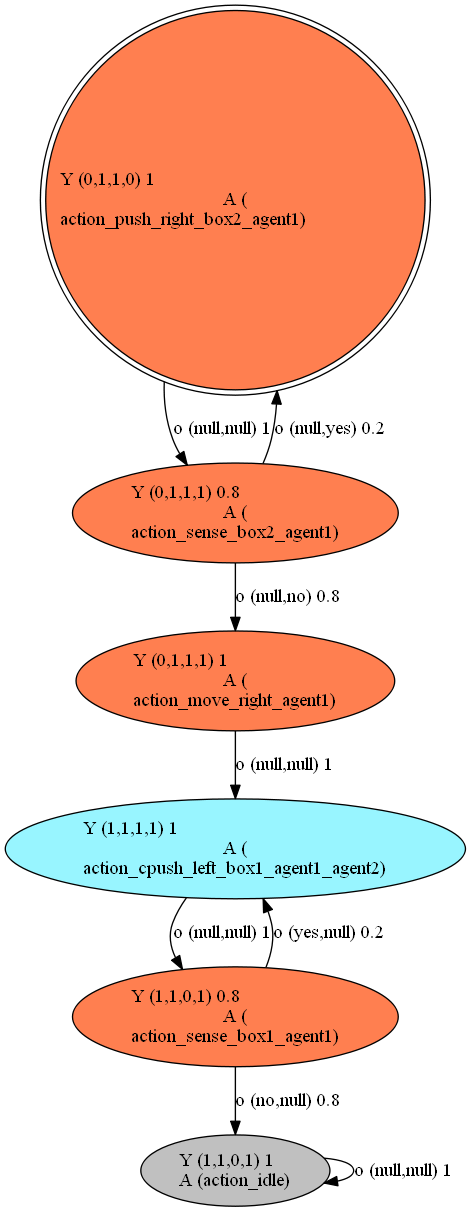
\includegraphics[width=0.25\textwidth,height=\textheight,keepaspectratio]{Agent1-Graph.dot.png}}
      \hfill
    \subfloat[After]{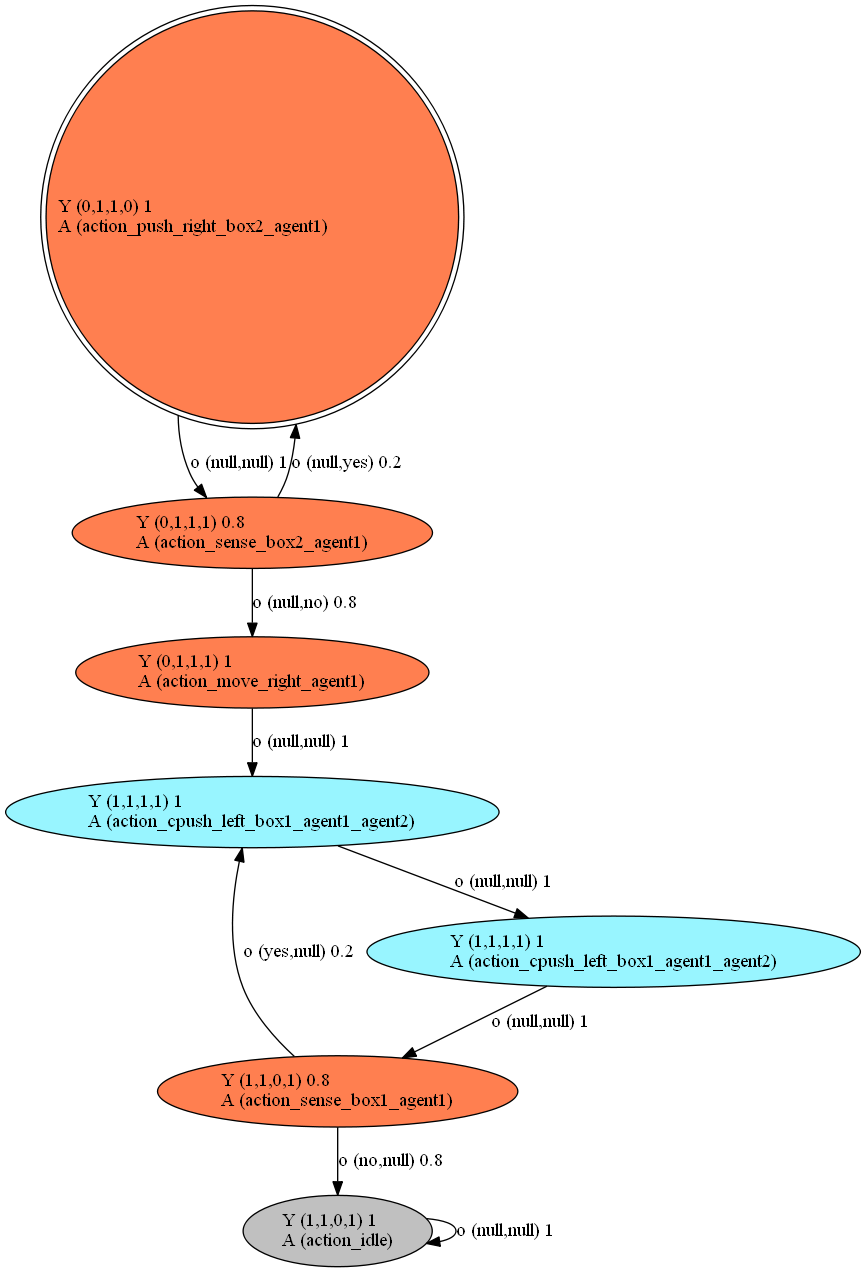
\includegraphics[width=0.45\textwidth,height=\textheight,keepaspectratio]{Agent1-Graph-Aligned.png}}
\caption{Write Caption Here}
\label{Fig:Alignment}
\end{figure}


% \begin{itemize}
%     \item We remove \emph{Agent1}'s simulation of \emph{Agent2}'s left movement.
%     \item The alignment algorithm inserts a {\em no-op} following \emph{Agent1}'s first sensing action, as the collaborative push in \emph{Agent2} occurs in depth 4.
%     \item We convert the first simulated push of \emph{Agent2} to a {\em no-op}.
%     \item We duplicate the collaborative push to avoid a live-lock. This way, even if \emph{Agent2} fails with his first push, it could still synchronize with \emph{Agent1} by entering the collaborative-push loop which ensures no live-lock can occur.
% \end{itemize}
\end{example}
}

\commentout{
\begin{algorithm}
\caption{Alignment Iteration}
\begin{algorithmic}[tbph]
\State Input: PolicyGraphs $G_1, ..., G_M$
\For{$G_i,  i\in\{1, ..., M\}$}
	\State {$\mathit{NoopsReqs} \gets \mathit{VertexToIntMapping}$}
      \State {$\mathit{CurrBFS} \gets \Call{BFS}{G_i}$}
      \While {$\mathit{CurrBFS.queue}$ is not empty}
	\State {$v \gets \mathit{CurrBFS.queue.pop}$}
	\State {$a \gets v.action$}
	\If {$a$ is public action}
	\State {$\mathit{identifier} \gets \Call{GetIdentifier}{v}$}
	\State {$\mathit{MaxNoop} \gets 0$}
	\For {$G_j,  j\in\{1, ..., M\}\setminus\{i\}$}
	\State {$\mathit{CurrNoop} \gets \Call{NoopReq}{G_j, \mathit{identifier}}$}
	\State {$\mathit{MaxNoop} \gets max(\mathit{MaxNoop}, \mathit{CurrNoop})$}
	\EndFor
	\State {$\mathit{NoopsReqs}[v] \gets \mathit{MaxNoop} - \mathit{CompensationTerm}$}
	\EndIf
	\EndWhile
	\State {$G_i' \gets \Call{AddNoops}{G_i, \mathit{NoopsReqs}}$}
\EndFor
\State {return $G_1', ..., G_M'$}
\end{algorithmic}
\end{algorithm}
}

\section{Empirical Study}

We provide experimental results focusing on longer planning horizons and scaling up with respect to current Dec-POMDP solvers.
The experiments were conducted on a variation of the popular cooperative box pushing problem.
We compare our algorithm, FDMAP, with two Dec-POMDP solvers, GMAA-ICE \cite{GMAAICE} and JESP \cite{JESP}, using MADP-tools. \cite{MADP}.
We evaluate FDMAP on a Windows machine with 4 cores of and 8GB of memory. We evaluate both GMMA-ICE and JESP on a Linux machine with 4 cores and 8GB of memory.


\subsection{\cbp}

We experiment with a variation of the well known cooperative box pushing domain, which emphasizes the need for a decentralized policy requiring coordination between agents and larger planning horizons, rather than good local reactive. In this problem, a cell can contain any number of agents and boxes. Each agent can move and push boxes in each of the four principle directions. Agents can also sense for a box at their location. Also, we require {\em no-op} actions for all agents.

All action except for the push actions are deterministic.
Light boxes can be pushed by a single agent, while heavy boxes can only be pushed by the collaborative push of two agents.
The goal of the agents is to move the boxes to a target tile, located at the upper left corner of the grid.
Initially, each box can appear in either the target tile (and hence, need not be moved) or the lower right tile, with equal probability.
Each action (except for {\em no-op}) has a cost --- 10 for moving, 1 for sensing (encouraging sensing rather than blindly pushing), 30 for pushing, and 20 for a collaborative push (per agent). The reward for moving a box to its target position is 500. In addition, there's a penalty of 10000 for pushing a box \emph{out} of the target tile to avoid abuse. In configurations with heavy boxes we double the reward and penalty.
A domain instance of $m$ tiles with $n$ agents, $l$ light boxes, and $h$ heavy boxes, has $m^{n+l+h}$ states, $(5\cdot(l+1)+4h\cdot(n-1))^n$ actions and $3^n$ observations.


\subsection{Settings} \eliran{separated to two different subsection, (Settings and Results), is it ok?}

We compared FDMAP with GMAA-ICE and DP-JESP. GMAA-ICE and DP-JESP, that require an horizon specification. Since FDMAP calculates a policy for an infinite horizon, the horizon parameter specifies the number of steps the policy was evaluated under.
For GMAA-ICE and DP-JESP we report the policy value as outputed from the algorithm. For FDMAP we measured the average discounted accumulated reward of 1000 simulations, where in each simulation the policy was run for the number of steps specified in the horizon column. 
\commentout{
The last horizon prefixed with Max is the maximal horizon measured for reaching the goal state in all simulations.}
\eliran{the commented out explanation above is not exact, I explained it at the end of the subsection.}

We demonstrate results on several configurations of \cbp. Each box starts at either the top-left or bottom-lower corner with equal probabilities. The problem name convention is composed of 5 marks, $\textit{BP}-[w][h][n][l][h]$.
Width, Height, Number of agents, Number of light boxes, Number of heavy boxes. For 1 dimensional grids, DP-JESP and GMAA-ICE were given with minimized version of the problem that do not include unnecessary actions | push and move for the up and down directions | to decrease the domain size. We specify the agents' initial locations (denoted by $I$), as well as the domain size, in the top row of each table.

GMAA-ICE and DP-JESP were given a 3600 seconds limit to solve each $\langle\textit{configuration, horizon}\rangle$ pair, FDMAP was given with the same amount to solve the problem once and output an infinite horizon solution. Each agent $i$ was given 900 seconds for  solving $P_i$. For the hardest problem configuration (BP-33221), we also present results for larger time limit, as 900 seconds were not sufficient for the agents to solve their $P_i$.

The time shown for GMAA-ICE is based only on its log in MADP-Toolbox, and does not include the problem loading, which is in many cases non negligible. FDMAP time does not include writing the SARSOP policies and graphs to disk, as they are highly dependent on hardware quality and can effectively remain in memory throughout the whole process.

In both GMAA-ICE and DP-JESP, configurations BP-32302, BP-32303 and BP-33221 could not be solved for a minimal horizon under the time limit. Therefore we provide comparisons only for the first four configurations, while harder configurations are shown in Table \ref{tbl:maxres}.

In DP-JESP, $\times$ marks a timeout. In GMAA-ICE we mark two different timeout options: FF refers to failure of finding a full policy for the required horizon, where FH refers to an earlier stage timeout when computing the heuristic function.

The planning horizons were chosen to allow for a minimally careful policy to be able to get all the boxes to their target tile. That is, the horizon should be large enough to allow the agents to sense the box at least once per tile that each box has to travel, and not force the agents into blindly pushing.
The last row prefixed with Max includes the results of the maximal successful planning horizons. We specify the horizons in parentheses in the Value entry. For FDMAP we also include the average number of steps, both measures are also presented in \ref{tbl:maxres} in their own columns (MaxSteps, AvgSteps).

\subsection{Results}

\begin{table}
\centering
\scriptsize
    % \caption{\guy{Use table instead of center, add labels and captions, refer to the tables in the text.}}
    \resizebox{\columnwidth}{!}{
    \begin{tabular}{||c|c|c|c|c|c|c||}
         \hline
         \multicolumn{7}{||c||}{BP-21210 $|S|=8, |A|=16, I=\langle(1,1),(1,2)\rangle$} \\
         \hline
         Horizon & \multicolumn{2}{|c|}{DP-JESP} & \multicolumn{2}{|c|}{GMAA-ICE} & \multicolumn{2}{|c||}{FDMAP}\\ 
         \hline
         & Time & Value & Time & Value & Time & Value \\
         \hline
         4 & 19.87 & 0 & 1.15 & 426.91 & 1.28 & 329.34 \\
         \hline
         5 & 1069.95 & 0 & 2.09 & 438.34 & " & 321.12 \\ 
         \hline
         6 & $\times$ & - & 6.97 & 448.19 & " & 337.63 \\
         \hline
         7 & $\times$ & - & 8.98 & 450.97 & " & 416.74 \\
         \hline
         Max & 1069.95 & 0 (5) & 8.71 & 453.73 (9) & " & 414.36 (21,4) \\
         \hline
    \end{tabular}
    }
    \caption{\label{tbl:small} Results for BP-21210. FDMAP outputs a reasonable value compared to GMAA-ICE, which most likely optimizes the small scaled problem.}
\end{table}

\begin{table}
\centering
\scriptsize
    \resizebox{\columnwidth}{!}{
    \begin{tabular}{||c|c|c|c|c|c|c||}
         \hline
         \multicolumn{7}{||c||}{BP-31211 $|S|=81, |A|=16, I=\langle(1,2),(1,3)\rangle$} \\
         \hline
         Horizon & \multicolumn{2}{|c|}{DP-JESP} & \multicolumn{2}{|c|}{GMAA-ICE} & \multicolumn{2}{|c||}{FDMAP}\\ 
         \hline
         & Time & Value & Time & Value & Time & Value \\
         \hline
         6 & $\times$ & - & FF & - & 2.03 & 245.18 \\
         \hline
         7 & $\times$ & - & FF & - & " & 298.07 \\
         \hline
         8 & $\times$ & - & FF & - & " & 344.76 \\
         \hline
         9 & $\times$ & - & FF & - & " & 359.78 \\
         \hline
         Max & 1861.30 & 279 (4) & 30.23 & 330.07 (4) & " & 590.82 (54,15) \\
         \hline
         \hline
         \multicolumn{7}{||c||}{BP-22202 $|S|=256, |A|=225,
         I=\langle(1,2),(2,2)\rangle$} \\
         \hline
         Horizon & \multicolumn{2}{|c|}{DP-JESP} & \multicolumn{2}{|c|}{GMAA-ICE} & \multicolumn{2}{|c||}{FDMAP}\\ 
         \hline
         & Time & Value & Time & Value & Time & Value \\
         \hline
         8 & $\times$ & - & FF & - & 3.88 & 267.26 \\
         \hline
         9 & $\times$ & - & FF & - & " & 241.61 \\
         \hline
         10 & $\times$ & - & FF & - & " & 259.77 \\
         \hline
         11 & $\times$ & - & FF & - & " & 237.91 \\
         \hline
         Max & 267.24 & 271 (3) & 160.18 & 320.46 (3) & " & 356.08 (23,9) \\
         \hline
         \hline
         \multicolumn{7}{||c||}{BP-22203 $|S|=1024, |A|=400,
         I=\langle(1,2),(2,2)\rangle$} \\
         \hline
         Horizon & \multicolumn{2}{|c|}{DP-JESP} & \multicolumn{2}{|c|}{GMAA-ICE} & \multicolumn{2}{|c||}{FDMAP}\\
         \hline
         & Time & Value & Time & Value & Time & Value \\
         \hline
         12 & $\times$ & - & FH & - & 21.01 & 269.85 \\
        \hline
         13 & $\times$ & - & FH & - & " & 264.87 \\
        \hline
         14 & $\times$ & - & FH & - & " & 272.20 \\
        \hline
         15 & $\times$ & - & FH & - & " & 304.49 \\
        \hline
         Max& 59.06 & 0 (2) & 1053.27 & 414 (2) & " & 518.02 (35,17) \\
         \hline
    \end{tabular}
    }
    \caption{\label{tbl:scale} FDMAP outperforms DP-JESP and GMAA-ICE with respect to both running time and policy value, when allowed to run for a large enough horizon. The running time is improved significantly.}
\end{table}


\begin{table}
\centering
\scriptsize
    \resizebox{\columnwidth}{!}{
    \begin{tabular}{||c|c|c|c|c|c||}
         \hline
         \multicolumn{6}{||c||}{FDMAP}\\ 
         \hline
         Problem & MaxSteps & AvgSteps & Time & Value & \%Wins\\
         \hline
         BP-32302 & & & & & \\
         $|S|=7776, |A|=3375$ & 40 & 14 & 92.70 & 243.91 & 100 \\
         $I=\langle(1,2),(1,3),(2,3)\rangle$ & & & & & \\
         \hline
         BP-32303 &&&&& \\
         $|S|=46656, |A|=8000$ & 43 & 21 & 1799.94 & 353.82 & 98 \\
         $I=\langle(1,2),(1,3),(2,3)\rangle$ & & & & & \\
         \hline
         BP-33221 &&&&& \\
         $|S|=59049, |A|=324$ & 124 & 37 & 2962.29 & 8.64 & 95 \\
         $I=\langle(1,3),(3,1)\rangle$ & & & & & \\
         \hline
         BP-33221 &&&&& \\
         3600 seconds per agent  & 105 & 35 & 5379.32 & 345.56 & 100 \\
         &&&&&\\
         \hline
    \end{tabular}}
    \caption{\label{tbl:maxres} Results for the largest scaled problems, which only FDMAP managed to solve. Running times are rapidly increasing while reaching the scales limit of the underlying POMDP solver. The policies are still very robust, and reach the goal state in most cases. (\%Wins) }
\end{table}

\begin{table}
\centering
\scriptsize
    \resizebox{\columnwidth}{!}{
    \begin{tabular}{||c|c|c|c|c|c|c||}
         \hline
         \multicolumn{7}{||c||}{BPPEN-13211 $|S|=81, |A|=16, I=\langle(1,1),(1,2)\rangle$} \\
         \hline
         Horizon & \multicolumn{2}{|c|}{DP-JESP} & \multicolumn{2}{|c|}{GMAA-ICE} & \multicolumn{2}{|c||}{FDMAP}\\ 
         \hline
         & Time & Value & Time & Value & Time & Value \\
         \hline
         6 & $\times$ & - & FF & - &  1.99 & 222.65 \\
         \hline
         7 & $\times$ & - &  FF & - & " & 289.98 \\
         \hline
         8 & $\times$ & - &  FF & - & " & 321.04 \\
         \hline
         9 & $\times$ & - &  FF & - & " & 373.80 \\
         \hline
         Max & 25.95 & 0 & 3537.67 & 438.95 (5) & " & 568.20 (53,15) \\
         \hline
         \hline
         \multicolumn{7}{||c||}{BPPEN-22202 $|S|=256, |A|=225,
         I=\langle(1,2),(2,2)\rangle$} \\
         \hline
         Horizon & \multicolumn{2}{|c|}{DP-JESP} & \multicolumn{2}{|c|}{GMAA-ICE} & \multicolumn{2}{|c||}{FDMAP}\\ 
         \hline
         & Time & Value & Time & Value & Time & Value \\
         \hline
         8 & $\times$ & - & FF & - & 3.72 & 231.3\\
         \hline
         9 & $\times$ & - & FF & - & " & 236.91 \\
         \hline
         10 & $\times$ & - & FF & - & " & 249.23 \\
         \hline
         11 & $\times$ & - & FF & - & " & 253.72 \\
         \hline
         Max & 495.61 & 135.40 (3) & 446.03 & 213.79 (3) & " & 289.55 (21,9) \\
         \hline
         \hline
         \multicolumn{7}{||c||}{BPPEN-22203 $|S|=1024, |A|=400,
         I=\langle(1,2),(2,2)\rangle$} \\
         \hline
         Horizon & \multicolumn{2}{|c|}{DP-JESP} & \multicolumn{2}{|c|}{GMAA-ICE} & \multicolumn{2}{|c||}{FDMAP}\\
         \hline
         & Time & Value & Time & Value & Time & Value \\
         \hline
         12 & $\times$ & - & FH & - & 14.67 & 294.64\\
        \hline
         13 & $\times$ & - & FH & - & " & 306.54 \\
        \hline
         14 & $\times$ & - & FH & - & " & 319.93 \\
        \hline
         15 & $\times$ & - & FH & - & " & 352.57 \\
        \hline
         Max& 38.70 & 0 (2) & 1054.5 & 326.504 (2) & " & 533.26 (37,15) \\
         \hline
    \end{tabular}
    }
    \caption{\label{tbl:bppen}Results for a variation of \cbp, in which we penalize an agent for pushing a light box blindly.}
\end{table}


\eliran{Should we bold the running times and max values in tables \ref{tbl:scale} and \ref{tbl:bppen}?}
Table \ref{tbl:small} shows that FDMAP manages to produce reasonable results compared to the other solvers even when dealing with extremely small domains, and present collaborative planning capabilities.

When scaling up the problems as shown in Table \ref{tbl:scale}, we can see that not only FDMAP manages to produce policies with higher quality, but also manages to reduce the planning time significantly. This is due to the fact that FDMAP does not plan directly on the decentralized model, but rather solves multiple POMDP models, which are known to require much less computational effort \cite{DECPOMDPCOMP}.

For the largest problems, as can be seen in Table \ref{tbl:maxres}, FDMAP still manages to produce good quality policies, yet with significant inclines in running time. The size of the hardest configuration, BP-33221, lies around the maximal scales reached by SARSOP \cite{SARSOP}.

To observe the difference between the policies FDMAP produces to the one GMAA-ICE does, we present another variation of the domain, where we add a penalty of 101 to light boxes push actions that occur with no box in the tile. The penalty is chosen to be slightly higher than the reward for pushing a box to the target tile, times the fail probability of the push action. Table \ref{tbl:bppen} presents the results (configuration name prefixed with BPPEN). We can see that the the reward difference on maximal results compared to Table \ref{tbl:scale} are much lower for FDMAP
\eliran{on BPPEN-13221, GMAA-ICE managed to produce result for higher horizon than in the original problem (5 instead of 4). This is the result I mailed you about, as I didn't manage to reproduce it and it is really close to the time limit, so I'm not sure it is valid} , indicating that FDMAP's policies in the non-penalty configurations exploit the horizon and avoid blindly pushing, leading to higher-quality results.

\commentout{
\section{Related Work}

\guy{This still requires work}
QDec-POMDPs~\cite{QDECPOMDP} are qualitative version of Dec-POMDPS that tackle a conceptually simpler, more structured, model. In QDec-POMDPs 
non-determinism replaces stochastic uncertainty. The model is factored (i.e., described at the level of state variables rather than states), and actions 
are described using preconditions and non-determinstic effects. Although QDec-POMDPs are also NEXT-Time hard, recent work in the area that leverages heuristic-search planners, has been able to scale up to much larger domains (e.g., box pushing on a grid of size 24,  12 agents and 12 boxes, implying a state space of $24^{24}$)
albeit, under the assumptions that actions are deterministic.

Dec-POMDP algorithms.
}

\section{Summary}
\eliran{should we add the future research or related work sections? I think that talking about reward shaping for quality improvement and converting to online POMDP and RL planners for scale are both interesting and easy to explain approaches}
We presented FDMAP --- an algorithm for solving factored Dec-POMDPs. FDMAP begins by solving a centralized POMDP, which we call the team POMDP, obtaining a team plan. Then, FDMAP creates agent specific POMDPs whose solutions encourage agents to complete their role in the team plan. The agent plans are then aligned for synchronization between the agents. We experiment with box pushing examples that require collaboration, showing that we can scale to much larger problems than current Dec-POMDP solvers, while computing a reasonable policy.

\commentout{
There are two direction in which we deem FDMAP can be improved, in both scalability and solution quality.
The use of online planners instead of SARSOP as the POMDP solver, can greatly improve the scale of solvable problems. The changes in terms of algorithm architecture are minor, as we merely need to be able to produce the single agent policy graphs using an online solver. \ronen{In fact, it seems we could use an RL algorithm here to generate a policy for each agent, as we can simulate as many traces as we wish.
In fact, we could use the RL algorithm to solve the team POMDP. This would generate the needed traces as well. We would learn incrementally
both the team solution and the single-agent solution. Using this idea, we could probably scale up to very large problems. In fact, we can use this
approach to do MA RL. If we can do the projections. What we need is a simulator that let's us control all the agents at once.}
In terms of solution quality, we aim at using more principled methods of reward shaping, that come from the worlds of reinforcement learning in forms of multi-objectivization \cite{REWARDSHAPING}.
Our goal would be to convert the concept of contexted actions |as defined in section 3.2| into objectives of each agent, while preserving optimality with respect to the decentralized problem.
}

\bibliography{bibilography.bib}
\bibliographystyle{aaai}
\end{document}